\documentclass{article}
\usepackage{tikz}
\usetikzlibrary{circuits.logic.US, positioning}
\begin{document}

\begin{center}
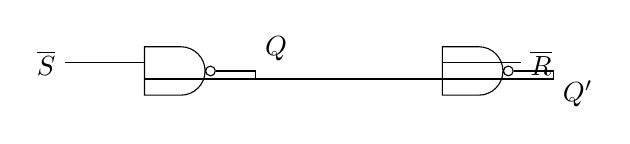
\begin{tikzpicture}[circuit logic US, logic gate inputs=nn, every node/.style={transform shape}, node distance=3cm]

  % NAND Gates
  \node[nand gate, draw, rotate=0] (G1) at (0,0) {};
  \node[nand gate, draw, rotate=0, right=of G1] (G2) {};

  % Inputs
  \draw (G1.input 1) -- ++(-1,0) node[left] {$\overline{S}$};
  \draw (G2.input 1) -- ++(1,0) node[right] {$\overline{R}$};

  % Cross-feedback
  \draw (G1.output) -- ++(0.5,0) |- (G2.input 2);
  \draw (G2.output) -- ++(0.5,0) |- (G1.input 2);

  % Outputs
  \draw (G1.output) -- ++(0.5,0) node[above right] {$Q$};
  \draw (G2.output) -- ++(0.5,0) node[below right] {$Q'$};

\end{tikzpicture}
\end{center}

\end{document}
